\chapter{Rahmenbedingungen}
    Forschungsgegenstand ist ein Reaktor, der im Rahmen des Verbundvorhabens \textbf{SCOORE} (Synthesis gas from recycling of CO$_2$) genutzt wurde. Ziel dieses Projekts ist es, eine CO$_2$-verbrauchende Synthesegasherstellung zu untersuchen und damit einen Beitrag zur Reduzierung der Treibhausgasemissionen in der chemischen Industrie zu leisten. 

    Das Vorhaben wird von der BASF~SE in Kooperation mit der Technischen Universität Bergakademie Freiberg durchgeführt und zielt darauf ab, eine großtechnisch umsetzbare Prozessführung für die nichtkatalytische Partialoxidation von Erdgas von Methan in einer CO$_2$ reichen Atmosphäre zu entwickeln \cite{Scoore_Enargus}.  
    \section{Reaktorgeometrie und Prozessbedingungen}
        Im Rahmen des Projekts wird der Prozess in zwei Varianten untersucht, um den Einfluss einer gezielten CO\textsubscript{2}-Zugabe auf die Reaktionsführung der nicht-katalytischen partiellen Oxidation (POx) von Erdgas systematisch zu bewerten. 
        
        Die erste Variante dient als \textbf{Referenzprozess} und beschreibt die konventionelle POx von Erdgas unter Standardbedingungen ohne zusätzliche CO\textsubscript{2}-Zugabe. Dieser Fall repräsentiert die typische industrielle Fahrweise, bei der Methan mit Sauerstoff und Wasserdampf unter stöchiometrisch limitierter Sauerstoffzufuhr zu einem kohlenmonoxid- und wasserstoffhaltigen Synthesegas umgesetzt wird. 
        
        In der zweiten Variante wird der Reaktionsverlauf unter vergleichbaren thermischen und stofflichen Betriebsbedingungen untersucht, jedoch mit einem zusätzlichen \textbf{CO\textsubscript{2}-Feed} im Zulauf. Durch die Einmischung von CO\textsubscript{2} verändert sich das lokale Reaktionsgleichgewicht sowie die Temperaturführung im Reaktor, wodurch sowohl kinetische als auch thermodynamische Effekte auftreten. 
        
        Der Vergleich beider Prozessführungen erlaubt Rückschlüsse auf den Einfluss des CO\textsubscript{2}-Gehalts auf die Flammenstabilität, die chemische Umwandlung der Reaktanden sowie die Zusammensetzung des Produktgases. Darüber hinaus wird untersucht, inwieweit die CO\textsubscript{2}-Zugabe zur Reduktion der Netto-CO\textsubscript{2}-Emissionen beiträgt und welche Anpassungen an Brennerdesign oder Betriebsparametern für eine stabile Prozessführung erforderlich sind.  
        
        In Tabelle \ref{tab:rahmenbedingungen_versuche} sind die wesentlichen \textbf{Prozessparameter und Betriebsbedingungen} der beiden Fälle zusammengefasst. Es ist ersichtlich, dass bei der CO\textsubscript{2}-Variante ein zusätzlicher Stoffstrom von etwa 196~kg/h Kohlendioxid in den Reaktor eingespeist wurde, während die übrigen Einsatzströme in Temperatur und Massenstrom nur geringfügig voneinander abweichen. Der Reaktor selbst weist ein Volumen von rund 134~Litern auf und wird unter adiabaten Bedingungen betrieben, wobei ein konstanter Wandwärmeverlust von etwa 30~kW berücksichtigt wird.
        
        \begin{table}[H]
            \centering
            \caption{Vergleich der Prozessfälle \cite{gonzales}}
            \label{tab:rahmenbedingungen_versuche}
            \begin{tabular}{llll}
            \toprule
            \textbf{Variablen} & & \textbf{Fall 1} & \textbf{Fall 2} \\
            \midrule
            \textbf{1. Erdgas} & Temperatur [°C] & 66,6 & 67,5 \\
                               & Massenstrom [kg/h] & 182,4 & 153,3 \\
            \midrule
            \textbf{2. Kohlendioxid} & Temperatur [°C] & -- & 67,5 \\
                                     & Massenstrom [kg/h] & 0 & 196,4 \\
            \midrule
            \textbf{3. Sauerstoff} & Temperatur [°C] & 231,9 & 231,2 \\
                                   & Massenstrom [kg/h] & 252,2 & 246,9 \\
            \midrule
            \textbf{4. Dampf} & Temperatur [°C] & 353,4 & 353,4 \\
                              & Massenstrom [kg/h] & 38,7 & 39,4 \\
            \midrule
            Wandwärmeverlust [kW] & & 30 & 30 \\
            Reaktorvolumen [L] & & 134 & 134 \\
            \midrule
            \textbf{Kommentar} & & Referenz & CO\textsubscript{2}-Zugabe \\
            \bottomrule
            \end{tabular}
        \end{table}
        
        Die Geometrie des Versuchreaktors und die Anordnung des Brenners sind in Abbildung \ref{fig:reaktorgeometrie} dargestellt. Der Reaktor besteht aus einem zylindrischen Hochtemperaturrohr, das mit einem gasdichten Stahlmantel und einer feuerfesten Ausmauerung versehen ist. Der Brenner ist als Mehrlochbrenner ausgeführt, um eine homogene Durchmischung der Einsatzgase und eine gleichmäßige Temperaturverteilung zu gewährleisten. Die Positionierung des Brenners am Reaktorkopf erlaubt eine definierte Einströmung der Reaktanden in die heiße Reaktionszone, wodurch charakteristische Temperaturgradienten entlang der Längsachse entstehen.
        
        \begin{figure}[H]
            \centering
            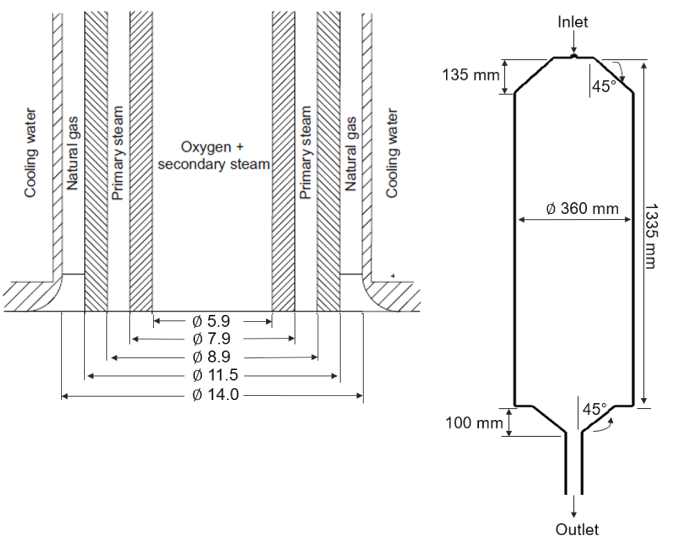
\includegraphics[width=0.8\linewidth]{img/sonstiges/Reaktorgeometrien.png}
            \caption{Geometrien des Reaktors sowie des Brenners}
            \label{fig:reaktorgeometrie}
        \end{figure}
        
        \section{Messwerte}
        Für beide in Tabelle \ref{tab:rahmenbedingungen_versuche} dargestellten Versuchsreihen wurden die \textbf{Synthesegaszusammensetzungen} sowie die \textbf{Temperaturen an verschiedenen Messpunkten im Reaktor} experimentell erfasst.  
        Die Lage der eingesetzten Thermoelemente ist in Abbildung \ref{fig:erweiterungen_messpunkte} dargestellt. Diese sind entlang der Reaktorlängsachse positioniert, um Temperaturverläufe innerhalb der Hauptreaktionszone und im Abgasbereich zu erfassen. Damit lassen sich lokale Temperaturmaxima und mögliche Rückzündungszonen identifizieren, was insbesondere für den Betrieb mit CO\textsubscript{2}-Zugabe von Bedeutung ist, da die Wärmekapazität und die Strahlungseigenschaften des Gases verändert werden.
        
        \begin{figure}[H]
            \centering
            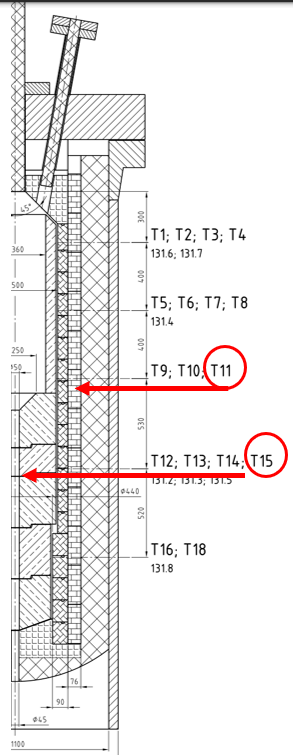
\includegraphics[width=0.2\linewidth]{img/Erweiterungen/Messpunkte.png}
            \caption{Messpunkte im Reaktor \cite{gonzales}}
            \label{fig:erweiterungen_messpunkte}
        \end{figure}
        
        Die gemessenen Synthesegaszusammensetzungen und Temperaturwerte sind in Tabelle \ref{tab:messwerte} zusammengefasst.  
        Beim Vergleich der beiden Fälle zeigt sich, dass die Zugabe von CO\textsubscript{2} zu einer leichten Erhöhung der Temperatur im Reaktorausgang sowie zu einer deutlichen Verschiebung der Gaszusammensetzung führt.  
        Der Wasserstoffanteil sinkt von etwa 60~Vol.-\% auf rund 42~Vol.-\%, während der CO-Anteil von 34~Vol.-\% auf 42~Vol.-\% ansteigt.  
        Das Verhältnis H\textsubscript{2}/CO reduziert sich damit von 1,76 auf 0,98, was auf eine verstärkte Umsetzung von Wasserstoff durch CO\textsubscript{2}-Verbrauchsreaktionen (z. B. Wasser-Gas-Shift oder CO\textsubscript{2}-Reformierung) schließen lässt.  
        Gleichzeitig steigt der CO\textsubscript{2}-Gehalt im Produktgas signifikant an, was auf eine unvollständige Umsetzung des zugegebenen Kohlendioxids hindeutet.
        
        \begin{table}[H]
            \centering
            \caption{Vergleich der Prozessfälle mit und ohne CO\textsubscript{2}-Zugabe \cite{gonzales}}
            \label{tab:messwerte}
            \begin{tabular}{l l c c}
            \toprule
             & \textbf{Einheit} & \textbf{Fall 1 (Referenz)} & \textbf{Fall 2 (CO\textsubscript{2}-Zugabe)} \\
            \midrule
            \textbf{Synthesegas (nass)} & kg/s & 0{,}13 & 0{,}18 \\
            \textbf{Temperatur Austritt} & °C & (1300)\textsuperscript{*} & (1342)\textsuperscript{*} \\
            Temperatur T102.11 & °C & 1407{,}4 & 1411{,}4 \\
            Temperatur T102.15 & °C & 1351{,}9 & 1371{,}6 \\
            \midrule
            H\textsubscript{2} & Vol.- trocken & 0{,}60 & 0{,}42 \\
            CO & Vol.- trocken & 0{,}34 & 0{,}42 \\
            CH\textsubscript{4} & Vol.- trocken & 0{,}01 & 0{,}00 \\
            CO\textsubscript{2} & Vol.- trocken & 0{,}05 & 0{,}15 \\
            \midrule
            H\textsubscript{2}/CO & – & 1{,}76 & 0{,}98 \\
            \bottomrule
            \end{tabular}
        \end{table}
        
        Die Messdaten zeigen somit, dass der zusätzliche CO\textsubscript{2}-Feed den Reaktionsverlauf signifikant beeinflusst.  
        Durch den erhöhten CO\textsubscript{2}-Anteil werden endotherme Reformierungsreaktionen begünstigt, was zu einer Veränderung der thermischen Bilanz und einer leichten Temperaturabsenkung in der Hauptreaktionszone führt.  
        Diese Ergebnisse bilden die Grundlage für die nachfolgende numerische Modellierung und Validierung der Reaktornetzwerke im Rahmen dieser Arbeit.
    \section{Vorbetrachtungen}
    \label{sec:vorbetrachtungen}
    
        Zur Vorbereitung der Modellierungsarbeiten liegen bereits umfangreiche CFD-Analysen sowie ein darauf basierendes komplexes Reaktornetzwerk-Modell (ROM) vor. 
        Diese Untersuchungen bilden die Grundlage für das Verständnis der Strömungs- und Reaktionsvorgänge innerhalb des betrachteten POx-Reaktors. 
        In Abbildung \ref{fig:reaktorsegmentierung} ist die CFD-basierte Segmentierung des Reaktors dargestellt, aus der das bestehende Netzwerk aus Perfectly Stirred Reactors (PSR) und Plug Flow Reactors (PFR) abgeleitet wurde.
        
        \begin{figure}[H]
            \centering
            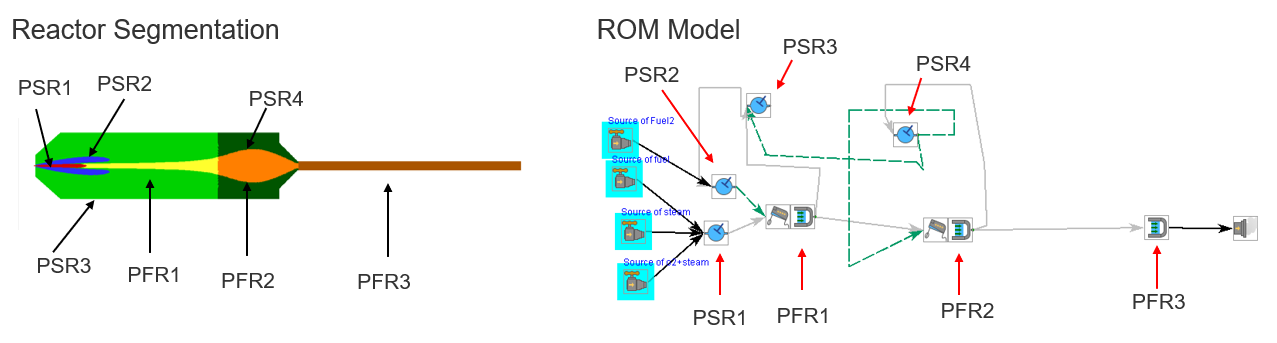
\includegraphics[width=1\linewidth]{img/sonstiges/Reactor Segmentation.png}
            \caption{Reaktorsegmentierung und komplexes ROM auf Basis einer CFD-Simulation \cite{gonzales}}
            \label{fig:reaktorsegmentierung}
        \end{figure}
    